%%% SVN stuff
\svnid{$Id: KNEAD_SSS_Appendix_B.tex 171 2025-04-27 02:23:43Z Lewis $}

\chapter{Data Flow Diagram Information}
\label{loc:DFD_Information}

This appendix provides information regarding the data flow diagrams used within this document.
The \DFD approach closely follows Yourdon Structured Method (\YSM) that is described in~\citeJESA.
The complete set of shapes required by the \YSM to effectively model a system are show in Figure~\ref{fig:YSM-DFD}.
\begin{figure}[htbp]
	\centering
			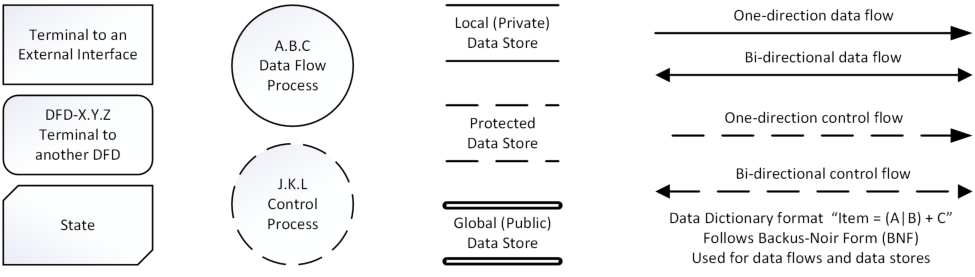
\includegraphics[width=6.5in]{images/YSM_DFD_Shapes_Image.pdf}%from LaTexInputs/images folder
		\caption{Yourdon Structured Method Data Flow Diagram Items}
	\label{fig:YSM-DFD}
\end{figure}
Minor alterations to the \YSM standard items are:
\begin{description}[itemindent=5pt,topsep=0pt,itemsep=0pt,partopsep=0pt, parsep=0pt]
	\item [Rounded Rectangle] represents a terminal to a higher-level \DFD. This is often represented as a square-corner rectangle but the rounded corners are preferred to more closely associate these terminators to the processes to which they attach, instead of true external terminators, which are traditionally depicted as squares or rectangles.
	\item [Protected Data Store] extends the \YSM to include object modeling. Thus, all three types of Object-Oriented Analysis \& Design (\OOAD) class types (private, protected, and public) can be modeled with this \YSM approach.
	\item [State] is represented as a rectangle with clipped upper left and lower-right corners so that the shape somewhat represents an ``S''. These usually have been denoted as either rectangles or circles, but this unique shape is preferred to minimize confusion between the \YSM \DFD items.
\end{description}

The interfaces between the items utilize the data flow representations shown in Figure~\ref{fig:YSM-DFD}.
These data flows may be color coded in the \DFDs within this document to more clearly identify the data flows.
Due to the limitations of human visual perception and display technology, the number of colors is limited so line patterns\footnote{The selected color and pattern choices should exclude black dashes since these are used for standard control flow. Black solid flows can be used but their definition should be made clear.} may be used to distinguish sub-types of data flows.
Not all color and line style patterns may be used on diagrams, but if needed, are listed below for reference.

% put line like 
%\input{../zProjectWideData/DFD_Dataflow_Colors.tex}% 
% to include project-specific colors and line patterns after general DFD description
